% opencolor-latex v1.0.0
% Author: Michele Piazzai
% Contact: michele.piazzai@uc3m.es
% License: MIT

\documentclass{standalone}

\usepackage{tikz}
\usetikzlibrary{calc}

\usepackage{etoolbox}
\usepackage{opencolor}

\newcommand\w{9em}
\newcommand\h{4.5em}

\begin{document}
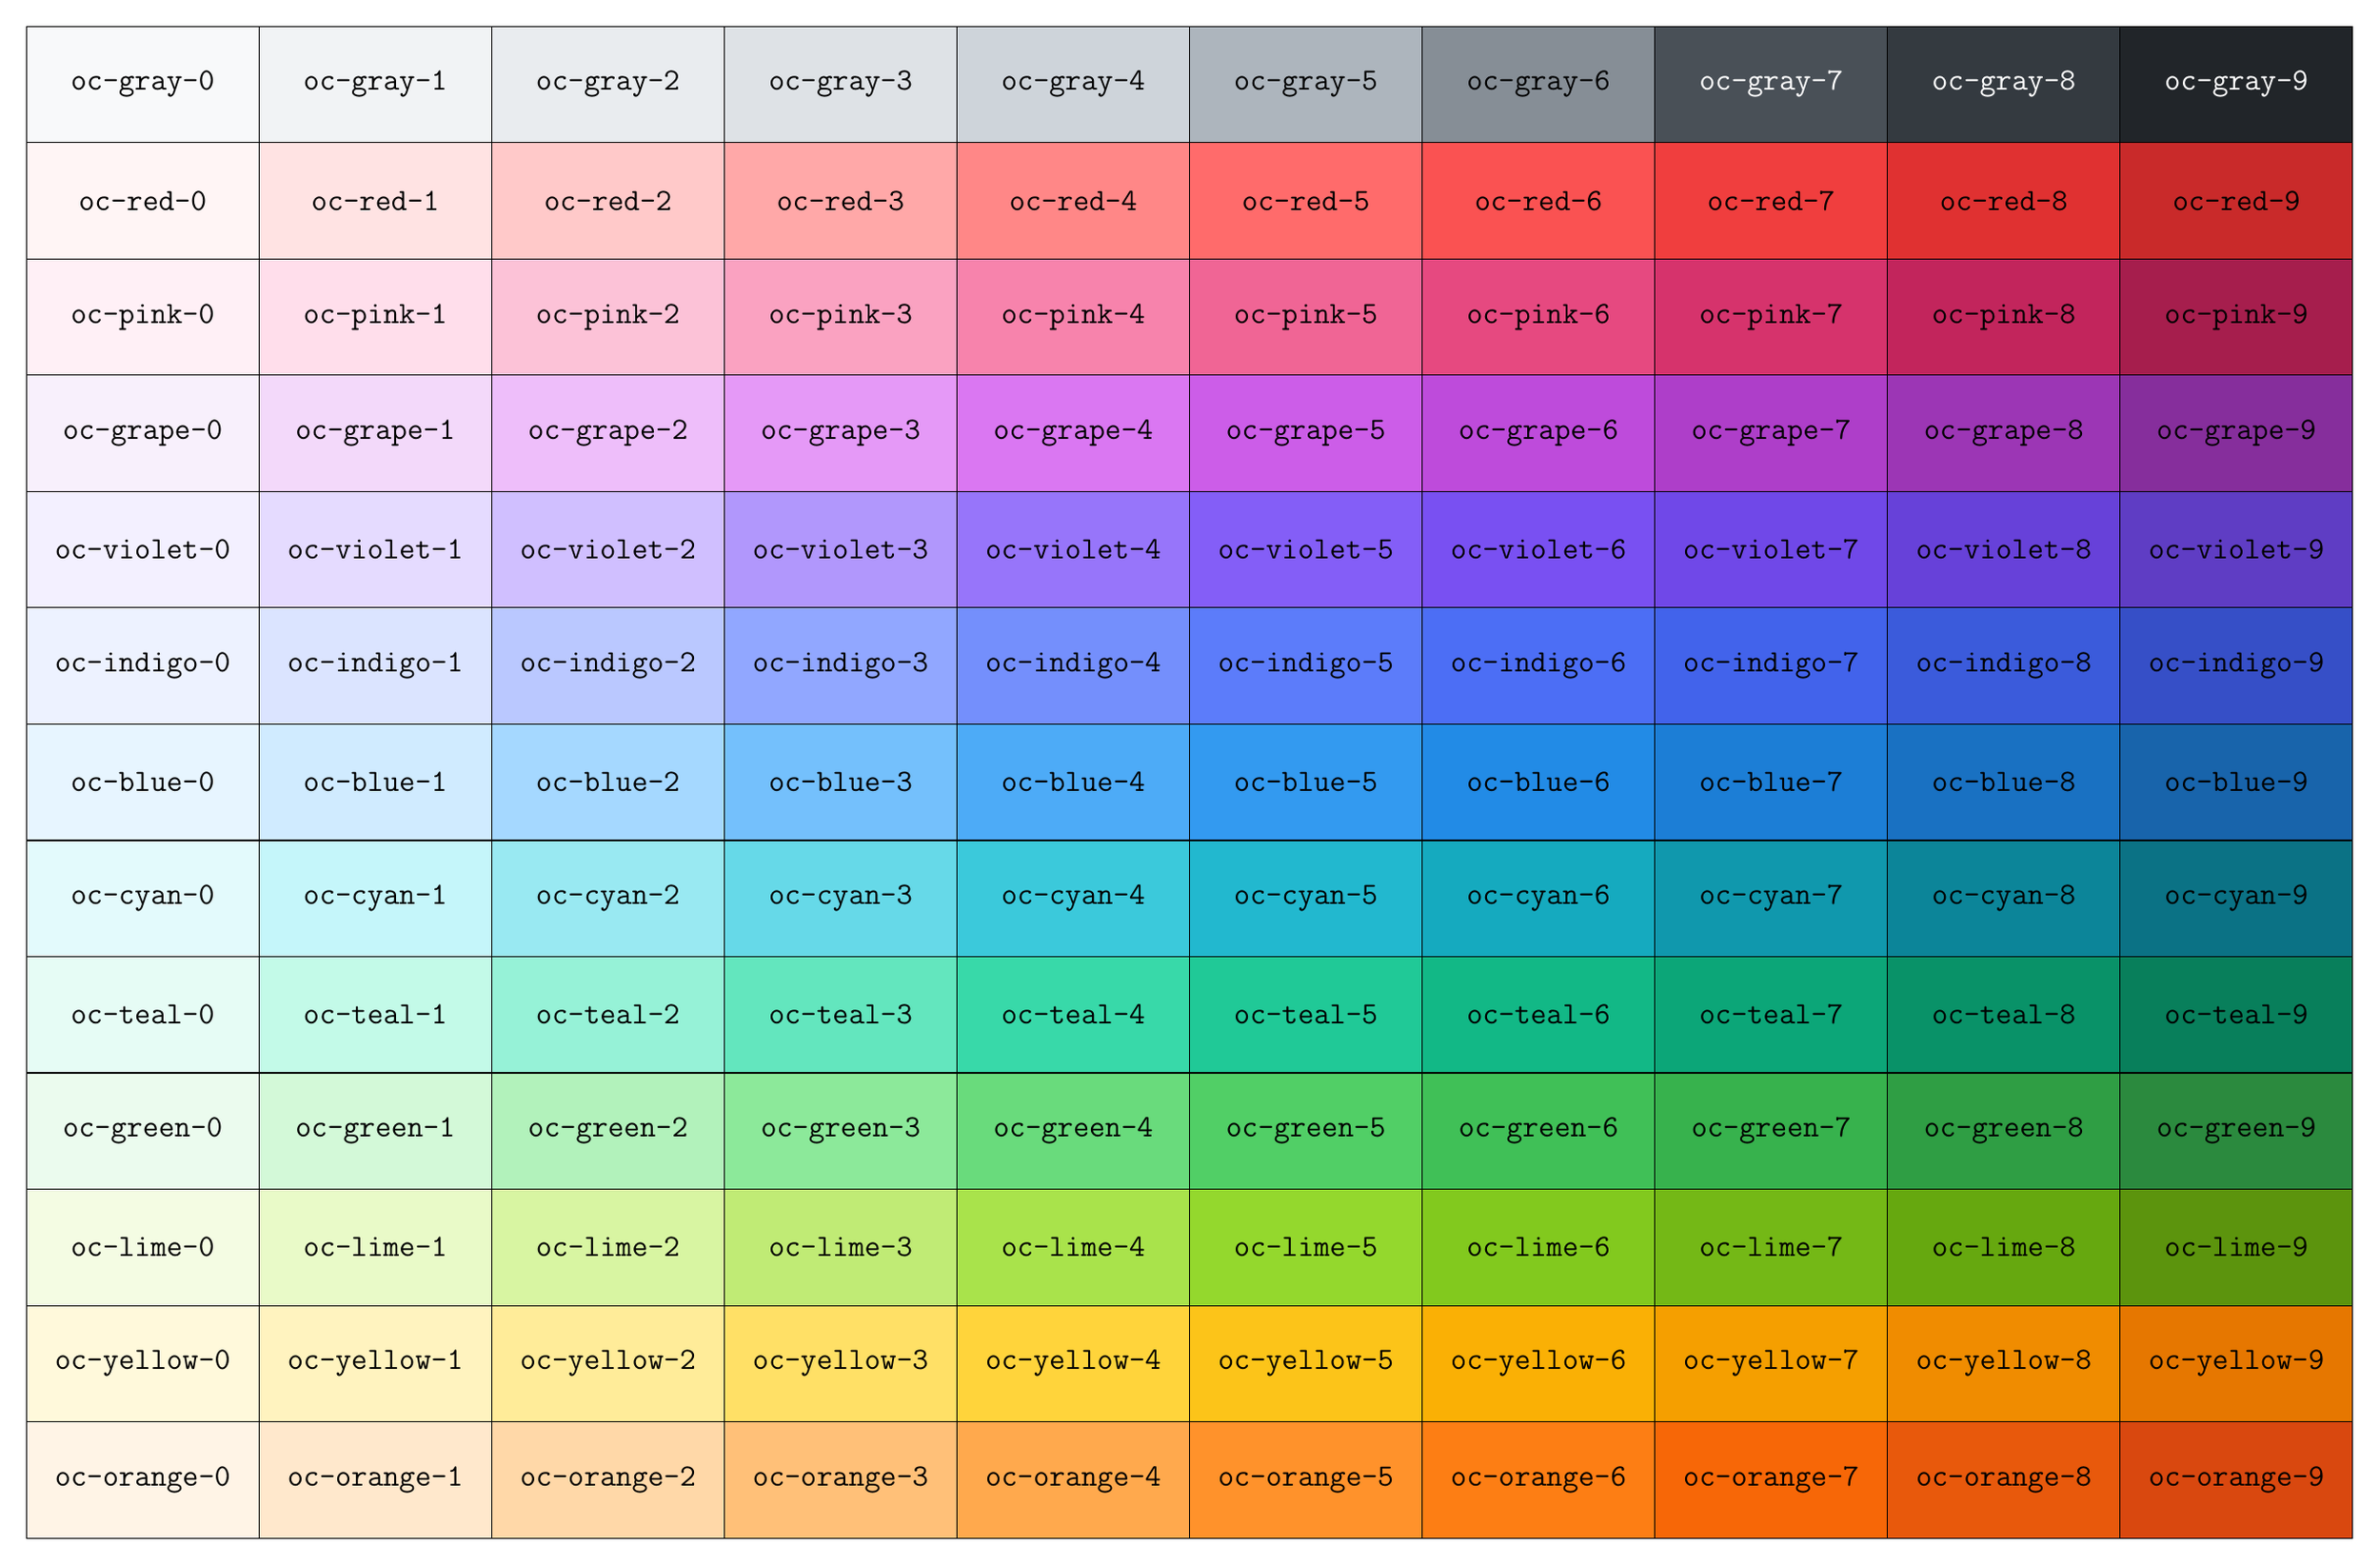
\begin{tikzpicture}
	\foreach \c [count=\x] in {gray,red,pink,grape,violet,indigo,blue,cyan,teal,green,lime,yellow,orange} {%
			\foreach \b in {0,...,9} {%
					\draw[\ifnumgreater{\x}{1}{black}{\ifnumgreater{\b}{6}{white}{black}}] (\b*\w,-\x*\h) node [draw=black,fill=oc-\c-\b,minimum width=\w,minimum height=\h] {\ttfamily\large oc-\c-\b};
				}
		}
\end{tikzpicture}

\end{document}
